% :Author: Stefan Kottwitz
% :Source: TeXblog - TikZ: shaded cube
%          http://texblog.net/latex-archive/graphics/tikz-cube-3d/
\documentclass[12pt]{article}
\usepackage{tikz}
\usepackage{verbatim}

\begin{comment}

:Title: Sudoku 3D cube
:Tags: 3D, Transformations

This example shows how to create an effective 3D effect using the ``slant`` transformation.
Shading has been added to enhance the 3D impression. Read more about this example over
at TeXblog_. 

.. _TeXblog: http://texblog.net/latex-archive/graphics/tikz-cube-3d/

:Author: Stefan Kottwitz
:Source: `TeXblog - TikZ: shaded cube`__

.. __: http://texblog.net/latex-archive/graphics/tikz-cube-3d/

\end{comment}

\usetikzlibrary{positioning}
\begin{document}
\large
\pagestyle{empty}
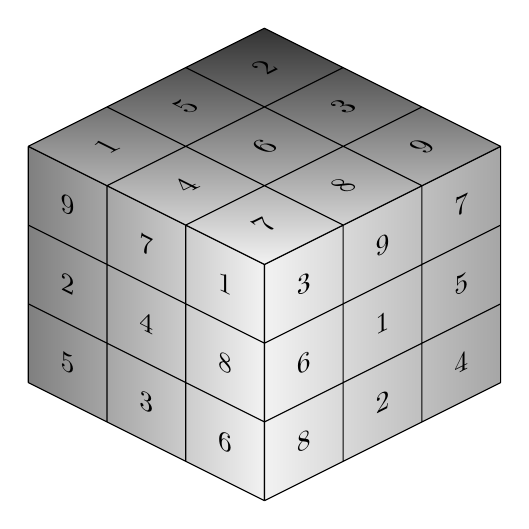
\begin{tikzpicture}[every node/.style={minimum size=1cm},on grid]
\begin{scope}[every node/.append style={yslant=-0.5},yslant=-0.5]
  \shade[right color=gray!10, left color=black!50] (0,0) rectangle +(3,3);
  \node at (0.5,2.5) {9};
  \node at (1.5,2.5) {7};
  \node at (2.5,2.5) {1};
  \node at (0.5,1.5) {2};
  \node at (1.5,1.5) {4};
  \node at (2.5,1.5) {8};
  \node at (0.5,0.5) {5};
  \node at (1.5,0.5) {3};
  \node at (2.5,0.5) {6};
  \draw (0,0) grid (3,3);
\end{scope}
\begin{scope}[every node/.append style={yslant=0.5},yslant=0.5]
  \shade[right color=gray!70,left color=gray!10] (3,-3) rectangle +(3,3);
  \node at (3.5,-0.5) {3};
  \node at (4.5,-0.5) {9};
  \node at (5.5,-0.5) {7};
  \node at (3.5,-1.5) {6};
  \node at (4.5,-1.5) {1};
  \node at (5.5,-1.5) {5};
  \node at (3.5,-2.5) {8};
  \node at (4.5,-2.5) {2};
  \node at (5.5,-2.5) {4};
  \draw (3,-3) grid (6,0);
\end{scope}
\begin{scope}[every node/.append style={
    yslant=0.5,xslant=-1},yslant=0.5,xslant=-1
  ]
  \shade[bottom color=gray!10, top color=black!80] (6,3) rectangle +(-3,-3);
  \node at (3.5,2.5) {1};
  \node at (3.5,1.5) {4};
  \node at (3.5,0.5) {7};
  \node at (4.5,2.5) {5};
  \node at (4.5,1.5) {6};
  \node at (4.5,0.5) {8};
  \node at (5.5,2.5) {2};
  \node at (5.5,1.5) {3};
  \node at (5.5,0.5) {9};
  \draw (3,0) grid (6,3);
\end{scope}
\end{tikzpicture}
\end{document}
